\begin{figure}
\begin{center}
    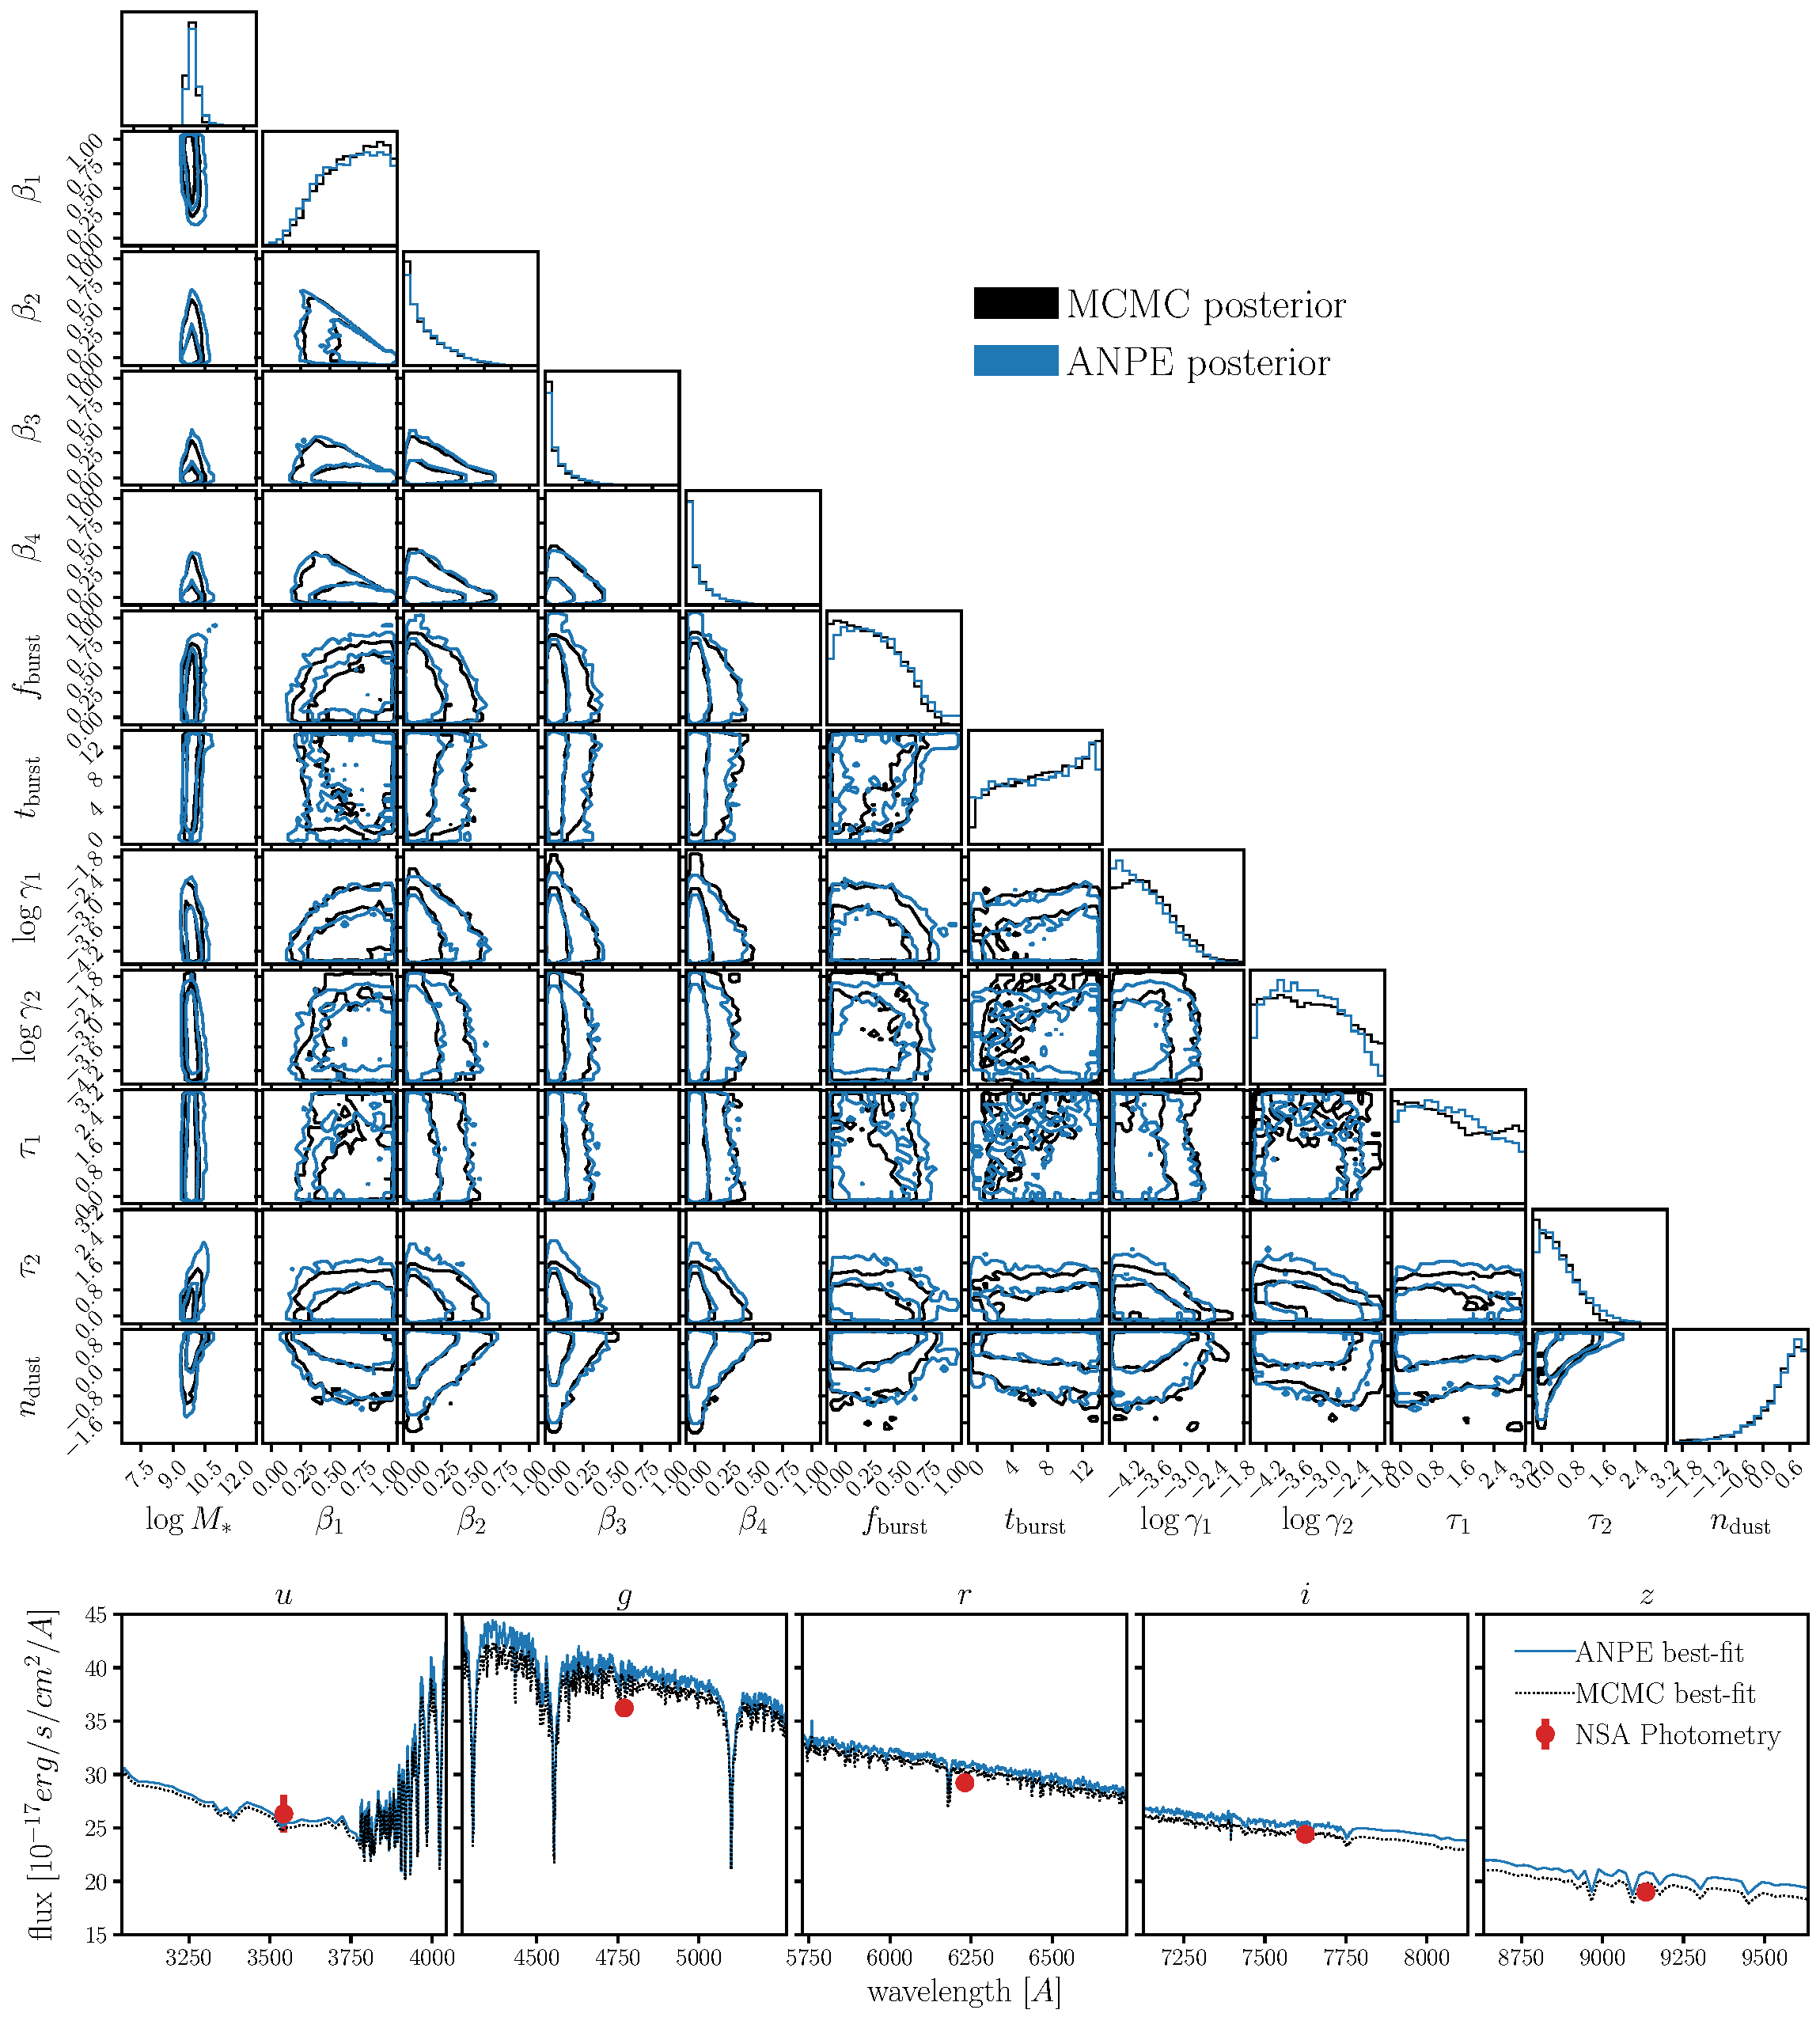
\includegraphics[width=0.9\textwidth]{figs/corner.pdf}
    \caption{\label{fig:corner}
    A comparison of the posteriors of the 12 SED model parameters derived from
    standard MCMC sampling (black) and ANPE (orange) for a randomly selected
    NSA galaxy.
    The posteriors are in excellent agreement for all of the parameters. 
    Estimating the posterior using MCMC sampling requires X hours. 
    Even using neural emulators to accelerate likelihood evaluations, MCMC
    sampling requires Y hours. 
    \emph{With ANPE, inferring the full posterior for a galaxy only requires 1
    second.}
    }
\end{center}
\end{figure}

\begin{figure}
\begin{center}
    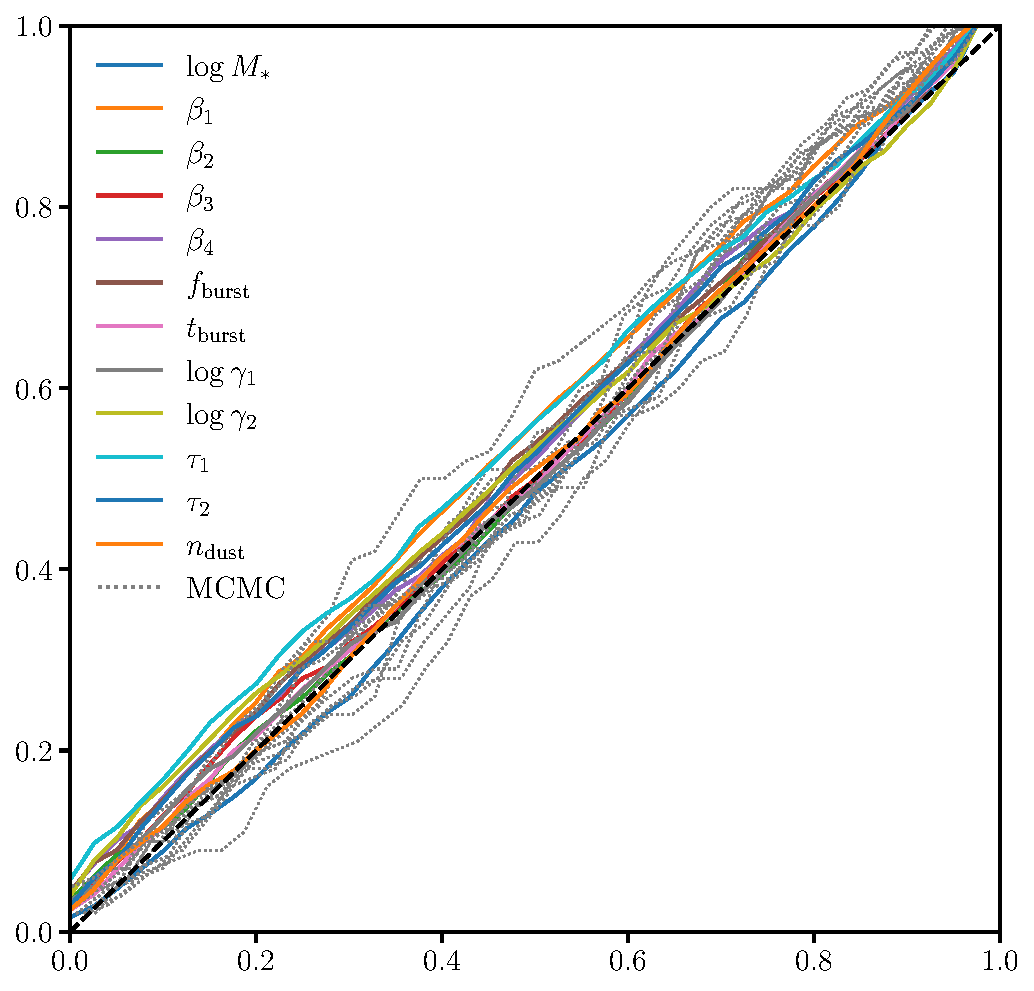
\includegraphics[width=0.5\textwidth]{figs/ppplot.pdf}
    \caption{\label{fig:pp}
    Probability-probability (p-p) plot of the ANPE for 1000 simulated test data. 
    For each SPS parameter, we plot the cumulative distribution function (CDF) of the
    percentile score of the true value within the ANPE marginalized posterior.
    For the true posteriors, the percentile score is uniformly distributed so
    the CDF is diagonal (black dashed).
    The test data is constructed in the same way as the training data
    (Section~\ref{sec:training}). 
    For reference, we include the p-p plot of the posterior estimated from MCMC
    sampling (gray). 
    \emph{The ANPE is in good agreement the true posterior.}
    }
\end{center}
\end{figure}

\begin{figure}
\begin{center}
    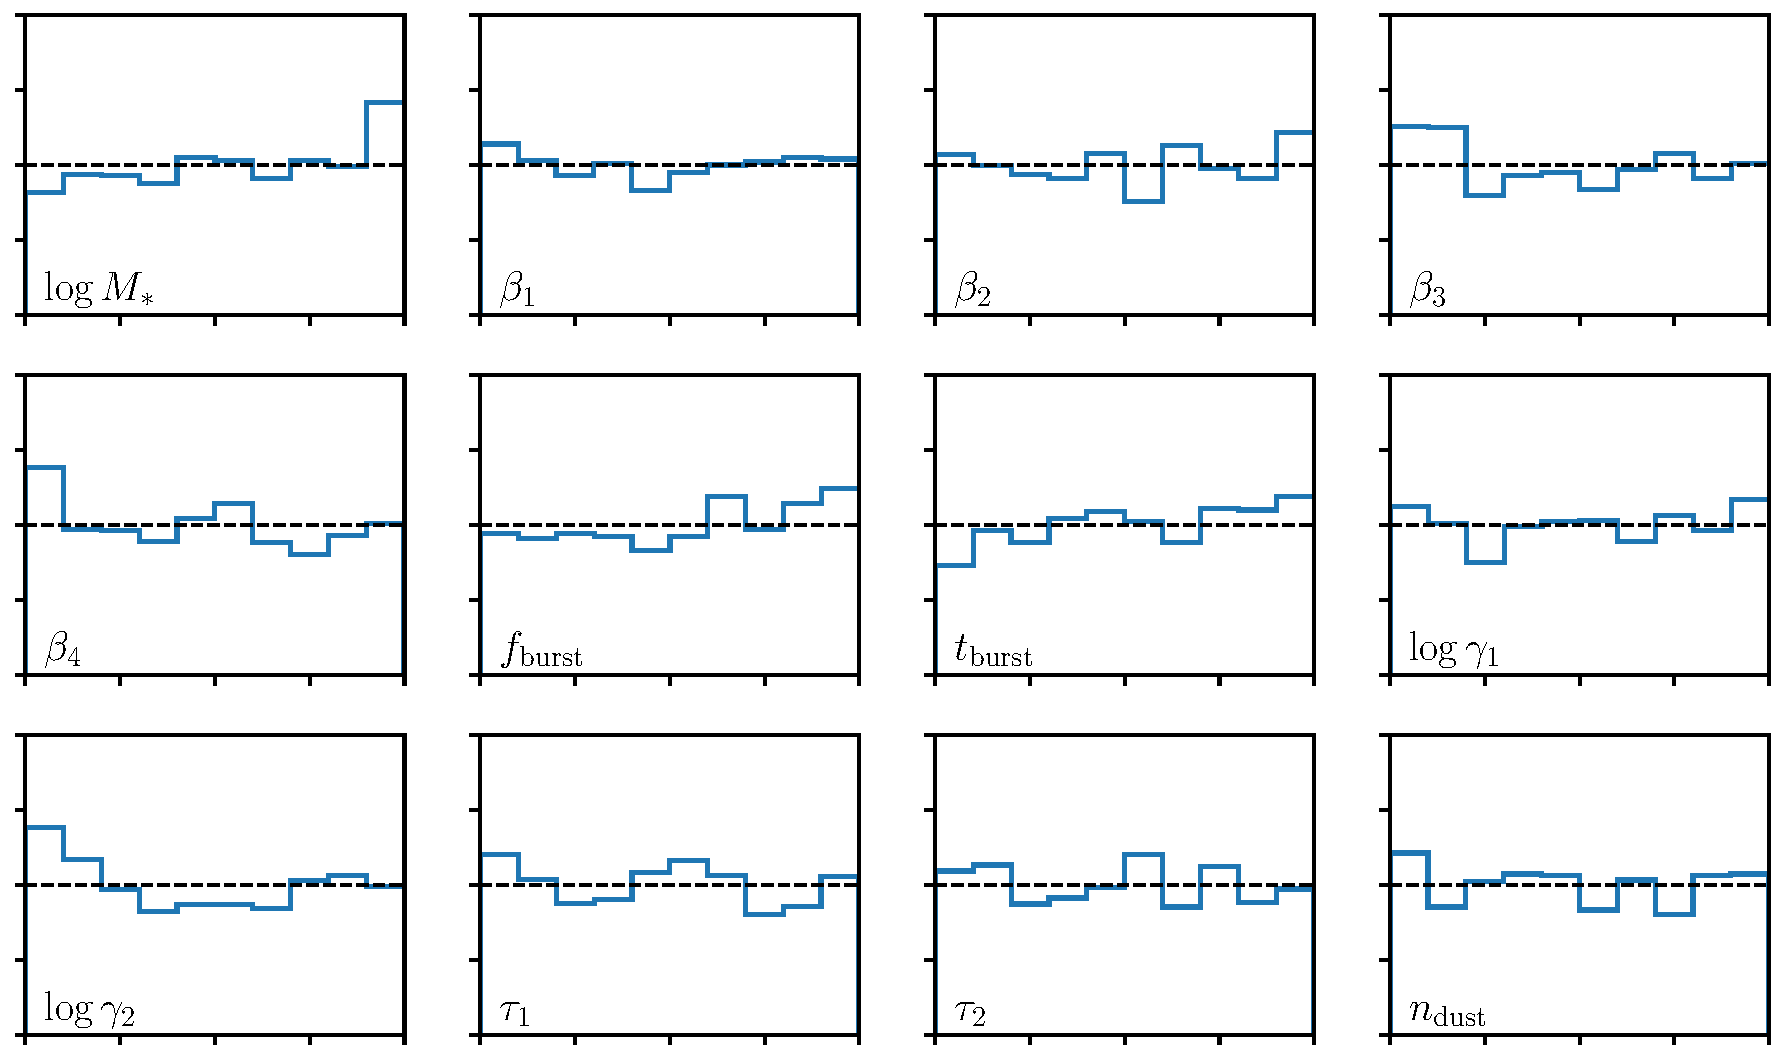
\includegraphics[width=0.9\textwidth]{figs/sbc.pdf}
    \caption{\label{fig:sbc}
    Simulation-based calibration plot of the ANPE for 1000 simulated test data. 
    For each SPS parameter, we plot the cumulative distribution function (CDF) of the
    percentile score of the true value within the ANPE marginalized posterior.
    For the true posteriors, the percentile score is uniformly distributed so
    the CDF is diagonal (black dashed).
    The test data is constructed in the same way as the training data
    (Section~\ref{sec:training}). 
    For reference, we include the p-p plot of the posterior estimated from MCMC
    sampling (gray). 
    \emph{The ANPE is in good agreement the true posterior.}
    }
\end{center}
\end{figure}
\section{Results} \label{sec:results}
\todo{validate the normaling flow SBI posteriors for a single case}  
compare the corner plot of a posterior derived from MCMC with the SBI 

\todo{validate the derived properties of galaxies for a handful of galaxies}


\todo{paragraph on the computational advantage}
